%
% Erstellt von Daniel Falkner
% daniel.falkner@akad.de
% 
\documentclass[xcolor=dvipsnames]{beamer}
\usepackage[T1]{fontenc}
\usepackage[utf8]{inputenc}
\usepackage[justification=centering,figurename=Abb.]{caption}

\usetheme{Warsaw}
\usecolortheme[named=YellowGreen]{structure}

\newcommand*{\Title}{Präsentation mit \LaTeX{}} %Titel
\subtitle{Modul ABC01} %Untertitel
\newcommand*{\Author}{Max Mustermann} %Name
\institute{AKAD Pinneberg} %Uni
\titlegraphic{
\includegraphics[scale=0.2]{akad_logo.png}} %Logo

\title{\Title}
\author{\Author}
\date{\today}

%Pdf Metainformationen
\subject{\Title}
\keywords{}

\begin{document}

%Titelseite
\begin{frame}
    \titlepage
\end{frame}

%Logo auf allen weiteren Folien
%\logo{
\includegraphics[scale=0.1]{akad_logo.png}}

%Inhaltsverzeichniss
\frame{\tableofcontents} 

%Ab hier die Folien 
 
\section{Text und Aufzählung}
\begin{frame} %%Eine Folie
  \frametitle{Ein Demotitel} %%Folientitel
  \framesubtitle{mit Untertitel} %%Fielenuntertitel
  \begin{block}{} 
    Text
  \end{block}
  \begin{block}{Aufzählung}
  	Viele Punkte
	  \begin{itemize}
  		\item Punkt 1
	  	\item Punkt 2
	  \end{itemize}
  \end{block}
\end{frame}

%\frame{\tableofcontents[currentsection]}

\section{Aufzählung}
\begin{frame}
  \frametitle{Diesmal eine Aufzählung über mehrere Folien}
	\begin{block}{Ich bin immer gleich}	
		\begin{itemize}[<+->]
			\item Punkt 1
			\item Punkt 2
			\item und der dritte Punkt
		\end{itemize}
	\end{block}
\end{frame}

\section{Texte}
\begin{frame}
  \frametitle{Diesmal Ein Text über mehrere Folien}
	Eine \pause sehr einfache Möglichkeit \pause über mehrere Seiten zu schreiben, \pause ist der  \texttt{pause} Befehl.
\end{frame}

\section{Unterabschnitte}
\begin{frame}
  \frametitle{mehreren Unterabschnitten}
  \framesubtitle{und einem Bild}
	\begin{figure}
	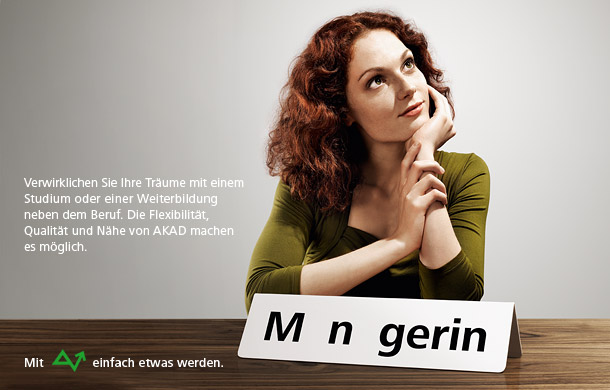
\includegraphics[scale=0.4]{akad_bild1.jpg}
			\caption{AKAD \\ \tiny{\textcolor{gray}{\url{http://www.akad.de}}}}
	\end{figure}
\end{frame}

\subsection{Lorem ipsum}
\begin{frame}
  \frametitle{Lorem ipsum}
  Lorem ipsum dolor sit amet, consetetur sadipscing elitr, sed diam nonumy eirmod tempor invidunt ut labore et dolore magna aliquyam erat, sed diam voluptua. At vero eos et accusam et justo duo dolores et ea rebum. Stet clita kasd gubergren, no sea takimata sanctus est Lorem ipsum dolor sit amet. Lorem ipsum dolor sit amet, consetetur sadipscing elitr, sed diam nonumy eirmod tempor invidunt ut labore et dolore magna aliquyam erat, sed diam voluptua. At vero eos et accusam et justo duo dolores et ea rebum. Stet clita kasd gubergren, no sea takimata sanctus est Lorem ipsum dolor sit amet.
\end{frame}

\subsection{Lorem ipsum kürzer}
\begin{frame}
  \frametitle{Lorem ipsum bisschen weniger}
  Lorem ipsum dolor sit amet, consetetur sadipscing elitr, sed diam nonumy eirmod tempor invidunt ut labore et dolore magna aliquyam erat, sed diam voluptua. At vero eos et accusam et justo duo dolores et ea rebum. Stet clita kasd gubergren, no sea takimata sanctus est Lorem ipsum dolor sit amet.
\end{frame}

\subsection{Lorem ipsum mit Rahmen}
\begin{frame}
  \frametitle{Lorem ipsum wieder mehr dafür mit anderen Rahmen}
  \begin{alertblock}{Lorem ipsum}
  Lorem ipsum dolor sit amet, consetetur sadipscing elitr, sed diam nonumy eirmod tempor invidunt ut labore et dolore magna aliquyam erat, sed diam voluptua. At vero eos et accusam et justo duo dolores et ea rebum. Stet clita kasd gubergren, no sea takimata sanctus est Lorem ipsum dolor sit amet. Lorem ipsum dolor sit amet, consetetur sadipscing elitr, sed diam nonumy eirmod tempor invidunt ut labore et dolore magna aliquyam erat, sed diam voluptua. At vero eos et accusam et justo duo dolores et ea rebum. Stet clita kasd gubergren, no sea takimata sanctus est Lorem ipsum dolor sit amet.
  \end{alertblock}
\end{frame}

\subsection*{Ende}
\begin{frame}
	\begin{block}{}	
		\begin{center}
			Vielen Dank für Ihre Aufmerksamkeit. \\
			\Author{}
		\end{center}	
	\end{block}
\end{frame}

\end{document}


